\documentclass[a4paper,12pt]{article}
\author{Adam Ilyas 725819 \\adam\_ilyas@mymail.sutd.edu.sg}
\title{
  CS-E4600 Algorithmic Methods of Data Mining
  Programming Project
}

\usepackage{verbatim}
\usepackage{amsmath,amsfonts,amssymb}
\usepackage{graphicx}
\usepackage[english]{babel}
\usepackage{listings}
\usepackage{amsmath}
\usepackage{listing}
\usepackage{algorithmicx}
\usepackage[noend]{algpseudocode}

\setlength\parindent{0pt}

\begin{document}
\vspace{8pt}
\maketitle

\section{Introduction}

The tasks you have to complete for the programming project are the following:
\begin{itemize}
\item[1. ] Design and implement your own graph-partitioning method;
\item[2. ] submit your solution, which should include the source code you developed and a report
 
\end{itemize}

We will use graphs from the Stanford Network Analysis Project (SNAP)

http://snap.stanford.edu/data/index.html

in particular, you can consider the following 5 collaboration networks:

\begin{lstlisting}
 ca-AstroPh, ca-CondMat, ca-GrQc, ca-HepPh, ca-HepTh
\end{lstlisting}

File formate
first line:

\begin{lstlisting}
# graphID numOfVertices numOfEdges k
\end{lstlisting}

Subsequent values:
\begin{lstlisting}
vertex1ID vertex2ID  
\end{lstlisting}

\section{Graph-partitioning task:}

Given an undirected graph $G = (V, E)$ and an integer
$k > 1$  
we want to partition the set of vertices $V$ into $k$ communities  
$V_1 , \dots, V_k$ so that $\cap_{i=1}^k V_i = V$
We want our communities $V_1 , \dots, V_k$ to be as much seperate from each other as possible. We also want the communities to have roughly equal size. 
Thus, we will evaluate the goodness of
a partition $V_1 , \dots, V_k$ by **minimizing** the objective function:
$$\phi(V_1 , \dots, V_k) = \frac{E(V_1 , \dots, V_k)}{\min_{1 \leq i \leq k} |V_i|}$$
where $E(V_1 , \dots, V_k)$ is the set of edges of G that is “cut” by the k communities: 
$$E(V_1 , \dots, V_k) = \{ (u,v) \in E \;| \; u \in V_i \text{ and } v \in V_j \text{ where } i \neq j \}$$

You should implement a program that reads a problem instance in the format specified above and
produces a partition $V_1 , \dots, V_k$ for which the objective function $\phi(V_1 , \dots, V_k)$ is as small as possible

\subsection{Algorithm 1: Unnormalized spectral clustering}

\textbf{Input}: graph adjacency matrix $A$, number $k$
\begin{itemize}
\item[1. ] form diagonal matrix $D$
\item[2. ] form unormalized Laplacian $L = D - A$
\item[3. ] compute the first $k$ eigenvectors $u_1 , \dots, u_k$ of $L$ (unnormalized Laplacian)
\item[4. ] form matrix $U \in \texttt{R}^{n \times k}$ with columns $u_1, \dots, u_k$
\item[5. ] consider the i-th row of $U$ as point $y_i \in \texttt{R}^k, \; i=1, \dots, n$
\item[6. ] cluster (kmeans) the points $\{y_i\}_{i=1, \dots, n}$ into clusters $C_1, \dots, C_k$
\end{itemize}

\textbf{output} clusters $A_1, \dots A_k$

\subsection{Algorithm 2: Normalized spectral clustering (generalized eigenproblem)}

\textbf{Input}: graph adjacency matrix $A$, number $k$
\begin{itemize}
\item[1. ] form diagonal matrix $D$
\item[2. ] form unormalized Laplacian $L = D − A$
\item[3. ] compute the first $k$ eigenvectors $u_1 , \dots, u_k$ of the
\textit{generalized eigenproblem} $L \mathbf{u} = \lambda D \mathbf{u}$
(eigenvectors of $L_{rw}$)
\item[4. ] form matrix $U \in \texttt{R}^{n \times k}$ with columns $u_1, \dots, u_k$
\item[5. ] consider the i-th row of $U$ as point $y_i \in \texttt{R}^k, \; i=1, \dots, n$
\item[6. ] cluster (kmeans) the points $\{y_i\}_{i=1, \dots, n}$ into clusters $C_1, \dots, C_k$
\end{itemize}

\textbf{output} clusters $A_1, \dots A_k$


\bigskip
This algorithm is similar to Algorithm 1. The difference is in

- step 3 where we find the
eigenvectors $u_1 , \dots, u_k$ of the
\textit{generalized eigenproblem} instead of the \textit{unnormalized laplacian}

$$L_{rw} := I - D^{-1} A$$

\subsection{Algorithm 3: Normalized spectral clustering (generalized eigenproblem, normalized U)}

This algorithm is the same as
Algorithm 2 but we \textit{normalize} $U$ so that rows have norm 1

\textbf{Input}: graph adjacency matrix $A$, number $k$
\begin{itemize}
\item[1. ] form diagonal matrix $D$
\item[2. ] form unormalized Laplacian $L = D − A$
\item[3. ] compute the first $k$ eigenvectors $u_1 , \dots, u_k$ of the
\textit{generalized eigenproblem} $L \mathbf{u} = \lambda D \mathbf{u}$
(eigenvectors of $L_{rw}$)
\item[4. ] form matrix $U \in \texttt{R}^{n \times k}$ with columns $u_1, \dots, u_k$
\item[5. ] \textit{normalize} $U$ so that rows have norm 1
\item[6. ] consider the i-th row of $U$ as point $y_i \in \texttt{R}^k, \; i=1, \dots, n$
\item[7. ] cluster (kmeans) the points $\{y_i\}_{i=1, \dots, n}$ into clusters $C_1, \dots, C_k$
\end{itemize}

\textbf{output} clusters $A_1, \dots A_k$

\subsection{Algorithm 4: Normalized spectral clustering (normalize U)}

\textbf{Input:} graph adjacency matrix $A$, number $k$

\begin{itemize}
\item[1. ] form diagonal matrix $D$
\item[2. ] form normalized Laplacian $L^\prime = I - D^{-1/2} A D^{-1/2}$

\item[3. ] compute the first $k$ eigenvectors $u_1 , \dots, u_k$ of $L^\prime$

\item[4. ] form matrix $U \in \texttt{R}^{n \times k}$ with columns $u_1, \dots, u_k$

\item[5. ] \textit{normalize} $U$ so that rows have norm 1
\item[6. ] consider the i-th row of $U$ as point $y_i \in \texttt{R}^k, \; i=1, \dots, n$
\item[7. ] cluster (kmeans) the points $\{y_i\}_{i=1, \dots, n}$ into clusters $C_1, \dots, C_k$
\end{itemize}

\textbf{Output:} clusters $A_1, \dots A_k$

This algorithm is similar to 
Algorithm 1. The difference is in

- step 2 we have \textit{normalized laplacian} instead of the \textit{unnormalized laplacian} $$L^\prime := I - D^{-1/2} A D^{-1/2}$$
- step 5 we \textit{normalize} $U$

\section{Performance}
We will use the following graphs to access the performance of the algorithms.
\begin{verbatim}
ca-HepTh ca-GrQc
\end{verbatim}

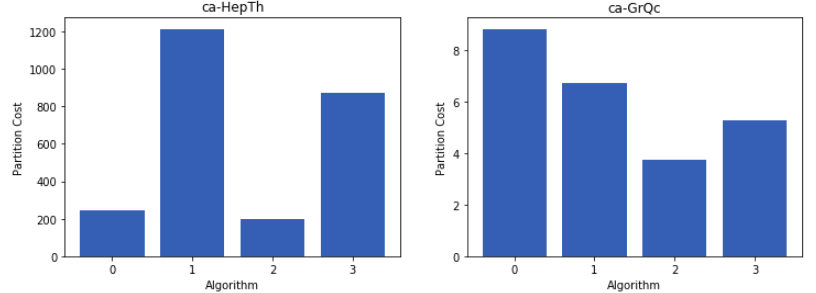
\includegraphics[width=\textwidth]{performance}

\begin{table}[h]
  \centering
\begin{tabular}{|l|l|l|l|l|}
\hline
Algo & 1 & 2 & 3 & 4 \\ \hline
\hline
\texttt{ca-HepTh} & 248.3 & 1214.0 & 198.8 & 871.9 \\ \hline
\texttt{ca-GrQc} & 8.8 & 6.7 & 3.7 & 5.26 \\ \hline
\end{tabular}
\end{table}

For both graphs, algorithm 3 has the lowest partition cost hence has the most balanced parition.
We will use Algorithm 3 : normalized spectral clustering (generalized eigenproblem, normalized U) to cluster our graph and produce the results.

\end{document}